\documentclass{article}

\usepackage[polish]{babel}
\usepackage{polski}
\usepackage[utf8]{inputenc}
\usepackage{longtable}
\usepackage{array}
\usepackage{enumitem}
\usepackage{makecell}
\usepackage{amsmath}
\usepackage{graphicx}
\usepackage{tikz}
\usepackage{float}
\usepackage{listings}
\usepackage[colorlinks=true, linkcolor=black]{hyperref}
\usepackage[letterpaper,top=2cm,bottom=2cm,left=3cm,right=3cm,marginparwidth=1.75cm]{geometry}

\renewcommand{\familydefault}{\sfdefault}

\definecolor{mygreen}{RGB}{117,167,117}
\definecolor{myred}{RGB}{255,1,1}
\definecolor{myblue}{RGB}{102,178,255}

\newcommand\myent[3]{%
\footnotesize%
$\begin{array}{@{}r@{}} 
#1 \\ #2 \\#3
\end{array}$%
}

\setcounter{tocdepth}{2}

\title{Projekt 2: Scenariusze działań \\ \large{Dokumentacja wstępna}}
\author{Damian Kąkol
	\and Piotr Komisarczyk
	\and Jan Kruszewski
	\and Aliaksandr Kulaha
	\and Kacper Leszczyński
	\and Michalina Majewska
	\and Adrian Rudź
	\and Jan Szablanowski}

\begin{document}
\maketitle
\tableofcontents

\newpage

\section{Cel projektu}
Celem projektu jest stworzenie aplikacji do definiowania i analizy systemów dynamicznych należących do pewnej klasy, będącej rozszerzeniem klasy systemów dynamicznych opisywanych językiem $\mathcal{AL}$.
Rozszerzenie to polega na dodaniu warunków o dowolnej długości czasu trwania akcji. W ramach projektu zostaną opracowane i zaimplementowane:
\begin{itemize}
	\item język akcji, który pozwoli na definiowanie scenariuszy systemów dynamicznych,
	\item język kwerend, który pozwoli na zadawanie pytań do zdefiniowanego scenariusza.
\end{itemize}	


\section{Język akcji}

\subsection{Opis języka \texorpdfstring{$\mathcal{AL}$}{AL}}
\label{sec:opis-jezyka-al}

Action Language $\mathcal{AL}$ to język formalny służący do modelowania systemów dynamicznych. Pozwala na reprezentację akcji, ich efektów oraz zależności czasowych pomiędzy nimi. $\mathcal{AL}$ zakłada liniowy model czasu i umożliwia analizę konsekwencji wykonywanych działań.

\subsubsection{Podstawowe założenia}
\begin{itemize}
    \item Prawo inercji
    \item Model czasu jest liniowy i dyskretny
    \item Akcje mają określony czas działania; podczas ich wykonywania wartości fluentów zmienianych przez te akcje są nieznane.
    \item Dynamiczne efekty akcji - jedna akcja może wywołać kolejną po upływie pewnego czasu od jej zakończenia.
    \item Sytuacja może wyzwalać akcje – niektóre stany mogą powodować wykonanie pewnych akcji.
\end{itemize}

\noindent Język $\mathcal{AL}$ spełnia powyższe założenia oraz dodatkowo zakłada, że każda akcja jest wykonywana w 1 jednostce czasu. W ramach projektu zostanie zaimplementowany język $\mathcal{AL}$ z dodatkowym założeniem o dowolnej długości czasu akcji. W następnych sekcjach zostanie opisana składnia $\mathcal{AL}$.

\subsubsection{Składnia języka $\mathcal{AL}$}

Podstawowe elementy języka $\mathcal{AL}$ to:
\begin{itemize}
    \item $F$ – zbiór fluentów, czyli zmiennych opisujących stan świata.
    \item $Ac$ – zbiór akcji, które mogą być wykonywane.
    \item Formuły logiczne – zdania określające warunki i efekty akcji.
\end{itemize}

\noindent W podstawowym języku $\mathcal{AL}$ wyróżnione są różne rodzaje zdań. Poniżej zostaną przedstawione możliwe zdania oraz ich zapis w języku $\mathcal{AL}$.
\begin{itemize}
    \item Gdy akcja $A$ znajdzie się w stanie spełniającym $\pi$, prowadzi do stanu spełniającego $\alpha$
    \begin{equation}
     A \text{ causes } \alpha \text{ if } \pi
    \end{equation}

    \item Akcja $A$ powoduje wykonanie akcji $B$ po $t$ chwilach czasu od zakończenia $A$, gdy zachodzi stan spełniający $\pi$
    \begin{equation}
        A \text{ invokes } B \text{ after } t \text{ if } \pi
    \end{equation}

    \item Gdy akcja $A$ znajdzie się w stanie spełniającym $\pi$ po jej wykonaniu wartość fluentu może, ale nie musi się zmienić
    \begin{equation}
        A \text{ releases } f \text{ if } \pi
    \end{equation}

    \item Gdy spełniony jest warunek $\pi$, akcja $A$ jest wykonywana.
    \begin{equation}
        \pi \text{ triggers } A
    \end{equation}
\end{itemize}

\subsubsection{Semantyka języka $\mathcal{AL}$}
Model $\mathcal{AL}$ to struktura:
\[S = (H, O, E)\]
Gdzie:
\begin{itemize}
    \item $H$ – funkcja historii stanów,
    \item $O$ – funkcja occlusion (określa, które fluenty mogą się zmieniać w wyniku akcji),
    \item $E$ – relacja określająca wystąpienia akcji.
\end{itemize}

\subsection{Rozszerzenie języka \texorpdfstring{$\mathcal{AL}$}{AL} o durations}
\label{sec:opis-jezyka-al-z-durations}

Poza podstawowymi założeniami zdefiniowanymi w sekcji \ref{sec:opis-jezyka-al}, język akcji zaimplementowany w ramach projektu będzie zawierał dodatkowe założenie o czasie trwania akcji. Każda akcja będzie opisana parą $(A, d)$, gdzie $A$ to nazwa akcja, a $d$ to czas trwania akcji.
\\ \\
Rozszerzony język akcji będzie dawał również możliwość zdefiniowania zdań o niemożliwości wykonania akcji w danym punkcie czasu albo przy zajściu pewnego warunku logicznego. 
\\ \\
Poniżej zostaną przedstawione możliwe zdania oraz ich zapis w w rozszerzonym języku $\mathcal{AL}$ o durations.
\begin{itemize}
    \item Gdy akcja $A$ o czasie trwania $d$ znajdzie się w stanie spełniającym $\pi$, prowadzi do stanu spełniającego $\alpha$
    \begin{equation}
     	(A, d) \text{ causes } \alpha \text{ if } \pi
    \end{equation}

    \item Akcja $A$ o czasie trwania $d_1$ powoduje wykonanie akcji $B$ (o czasie trwania $d_2$) po $t$ chwilach czasu od zakończenia $A$, gdy zachodzi stan spełniający $\pi$
    \begin{equation}
    	(A, d_1) \text{ invokes } (B, d_2) \text{ after } t \text{ if } \pi
    \end{equation}

    \item Gdy akcja $A$ o czasie trwania $d$ znajdzie się w stanie spełniającym $\pi$ po jej wykonaniu wartość fluentu może, ale nie musi się zmienić
    \begin{equation}
        (A, d) \text{ releases } f \text{ if } \pi
    \end{equation}

    \item Gdy spełniony jest warunek $\pi$, akcja $A$ o czasie trwania $d$ jest wykonywana.
    \begin{equation}
        \pi \text{ triggers } (A, d)
    \end{equation}

	\item Akcja $A$ o czasie trwania $d$ nie może być wykonana w chwili $t$.
    \begin{equation}
		\text{impossible } (A, d) \text{ at } t
    \end{equation}

	\item Akcja $A$ o czasie trwania $d$ nie może być wykonana, gdy spełniony jest warunek $\pi$.
	\begin{equation}
		\text{impossible } (A, d) \text{ if } \pi
	\end{equation}
\end{itemize}

\section{Scenariusze działań}
Scenariuszem nazywamy parę $Sc = (Obs, Acs)$, gdzie:
\begin{itemize}
	\item $Obs$ to zbiór obserwacji $Obs = {(\alpha_1, t_1), \ldots, (\alpha_n, t_n)}$, czyli zbiór formuł $\alpha_i$, które są obserwowane w trakcie realizacji scenariusza w czasie $t_i$.
	\item $Acs$ to zbiór akcji o określonym czasie trwania $Acs = {((A_1, d_1), t_1), \ldots, ((A_n, d_n), t_n)}$, które są wykonywane w trakcie realizacji scenariusza w czasie $t_i$.
\end{itemize}

\noindent Dodatkowo w scenariuszach rozważanych w projekcie mogą występować akcje nienależące do zbioru $Acs$, które są efektem wykonania innych akcji. W ramach projektu scenariusze będą definiowane w języku akcji z durations, opisanym w sekcji \ref{sec:opis-jezyka-al-z-durations}.

\section{Język kwerend}

\subsection{Opis}
Język kwerend pozwala na zadawanie pytań w danej klasie systemów dynamicznych. Kwerenda to zdanie logiczne. Mówimy, że kwerenda jest spełniona, gdy przyjmuje wartość prawdziwą.

W ramach projektu zostanie zaimplementowany język kwerend, który pozwoli na uzyskanie odpowiedzi na następujące pytania:
\begin{itemize}
    \item \textbf{Czy scenariusz $Sc$ jest możliwy do realizacji?}\\
    Scenariusz $Sc$ jest możliwy do realizacji, jeśli istnieje dla niego model w zadanej dziedzinie.
    \item \textbf{Czy w chwili $t$ realizacji scenariusza $Sc$ zawsze/kiedykolwiek wykonywana jest akcja $A$?}\\
    Przyjmuje się, że akcja $A$ jest wykonywana w chwilach $t_0+1$, $t_0+2$, \ldots, $t_0+d$,\\
    gdzie $t_0$ to początek trwania akcji, a $d$ to długość jej trwania.\\
    Akcja $A$ jest wykonywana zawsze, jeśli jest wykonywana w chwili $t$ realizacji scenariusza $Sc$ w każdym możliwym modelu.\\
    Akcja $A$ jest wykonywana kiedykolwiek, jeśli istnieje model, w którym jest wykonywana w chwili $t$ realizacji scenariusza $Sc$.
    \item \textbf{Czy w chwili $t \ge 0$ realizacji scenariusza $Sc$ warunek $\gamma$ zachodzi zawsze/kiedykolwiek?}\\
    Warunek $\gamma$ zachodzi zawsze, jeśli jest spełniony w chwili $t$ realizacji scenariusza $Sc$ w każdym możliwym modelu.\\
    Warunek $\gamma$ zachodzi kiedykolwiek, jeśli istnieje model, w którym jest spełniony w chwili $t$ realizacji scenariusza $Sc$.
\end{itemize}

\subsection{Dodatkowe założenia}
Przyjmuje się, że:
\begin{itemize}
    \item Akcje nie mogą zaczynać się w czasie $t < 0$. Zapytania o stan systemu sprzed chwili $t = 0$ są uznawane za niepoprawne. Ponadto warto zauważyć, że akcje mogą rozpoczynać się w chwili $t = 0$, jednak żadna akcja nie może być wykonywana w chwili $t = 0$.
    \item Od momentu zakończenia ostatniej akcji, stan systemu pozostaje niezmieniony. Zapytanie o stan dla danego scenariusza $Sc$ i modelu $M$ w chwili $t > t_{end}$, gdzie $t_{end}$ - moment zakończenia ostatniej akcji, jest równoważne z zapytaniem o stan w chwili $t_{end}$.
\end{itemize}

\subsection{Składnia języka kwerend}
\begin{itemize}
    \item $Possibly\ Sc$ – zapytanie o możliwość realizacji scenariusza $Sc$.
    \item $Always\ A\ at\ t\ when\ Sc$ – zapytanie, czy w chwili $t$ realizacji scenariusza $Sc$ zawsze wykonywana jest akcja $A$.
    \item $Possibly\ A\ at\ t\ when\ Sc$ – zapytanie, czy w chwili $t$ realizacji scenariusza $Sc$ kiedykolwiek wykonywana jest akcja $A$.
    \item $Always\ \gamma\ at\ t\ when\ Sc$ – zapytanie, czy w chwili $t$ realizacji scenariusza $Sc$ warunek $\gamma$ zachodzi zawsze.
    \item $Possibly\ \gamma\ at\ t\ when\ Sc$ – zapytanie, czy w chwili $t$ realizacji scenariusza $Sc$ warunek $\gamma$ zachodzi kiedykolwiek.
\end{itemize}

\section{Przykłady}
% TODO: Piotr

\subsection{Jan pijący kawę}
Na początku Jan jest śpiący, nie ma kawy i jest w domu.
Gdy jest śpiący, to śpi przez 2 jednostki czasu.
Po obudzeniu się, jeśli nie ma kawy, to typowo ją parzy.
Po zaparzeniu kawy, typowo ją pije.

\begin{enumerate}
    \item initially sleepy, -hasCoffee, atHome
    \item sleepy triggers Jan Sleep  
    \item Jan Sleep causes -sleepy after 2  
    \item typically -hasCoffee triggers Jan BrewCoffee at 2  
    \item Jan BrewCoffee causes hasCoffee  
    \item typically hasCoffee triggers Jan DrinkCoffee at 3  
    \item Jan DrinkCoffee causes energetic  
\end{enumerate}



\begin{tikzpicture}[x=1.5cm]
    \draw[mygreen,->,thick,>=latex]
      (0,0) -- (5,0) node[below right] {$\scriptstyle t$};
    \foreach \Xc in {0,...,4}
    {
      \draw[mygreen,thick] 
        (\Xc,0) -- ++(0,5pt) node[above] {$\scriptstyle \Xc$};
    }
    
    % Sleep trwa 2 jednostki czasu (0-1)
    \fill[myred] 
        ([xshift=5pt]0,0.25)  
          rectangle node[above] {\strut\small Sleep} 
        ([xshift=-5pt]2,0.35);  

    % BrewCoffee w czasie 2
    \fill[myred] 
        ([xshift=5pt]2,0.50)  
          rectangle node[above] {\strut\small BrewCoffee} 
        ([xshift=-5pt]3,0.60);  

    % DrinkCoffee w czasie 3
    \fill[myred] 
        ([xshift=5pt]3,0.75)  
          rectangle node[above] {\strut\small DrinkCoffee} 
        ([xshift=-5pt]4,0.85);  

    \node[below,align=left,anchor=north,inner xsep=0pt,color=myred] 
      at (0,0) 
      {\myent{s}{\neg c}{h}};  
    \node[below,align=left,anchor=north,inner xsep=0pt] 
      at (1,0) 
      {\myent{s?}{c?}{h?}};  
    \node[below,align=left,anchor=north,inner xsep=0pt] 
      at (2,0) 
      {\myent{\neg s}{\color{myred}\neg c\ast}{h?}};  
    \node[below,align=left,anchor=north,inner xsep=0pt] 
      at (3,0) 
      {\myent{\neg s}{\color{myred}c\ast}{h?}};  
    \node[below,align=left,anchor=north,inner xsep=0pt] 
      at (4,0) 
      {\myent{\neg s}{c?}{\color{myred}e\ast}};  
\end{tikzpicture}

\subsection{Ewa czytająca książkę}

Na początku Ewa jest zmęczona, nie ma książki, jest w domu i biblioteka jest zamknięta. Ewa odpoczywa przez 1 jednostkę czasu, co sprawia, że przestaje być zmęczona. Następnie, przez kolejną jednostkę czasu, pije kawę, co sprawia, że staje się energiczna. W czasie 3 biblioteka się otwiera. Jeśli Ewa nie zamówiła książki przez internet, w czasie 4 idzie do biblioteki, aby ją wypożyczyć. W czasie 5, jeśli ma książkę, zaczyna ją czyta

\begin{enumerate}
    \item initially tired, -hasBook, atHome, -atLibrary, -isLibraryOpen

    \item tired triggers Ewa Rest
    \item Ewa Rest causes -tired after 1
    \item typically -tired triggers Ewa DrinkCoffee at 1
    \item Ewa DrinkCoffee causes energetic
    \item isLibraryOpen at 3
    \item -isLibraryOpen at 6
    \item typically -hasBook and atHome triggers Ewa GoToLibrary at 4
    \item Ewa GoToLibrary causes -atHome, atLibrary
    \item typically atLibrary and -hasBook triggers Ewa BorrowBook
    \item Ewa BorrowBook causes hasBook if atLibrary, -hasBook
    \item hasBook typically causes Ewa ReadBook at 5
\end{enumerate}

\begin{tikzpicture}[x=1.8cm]  % Zmniejszenie jednostki dla formatu A4
    % Oś czasu
    \draw[mygreen,->,thick,>=latex]
      (0,0) -- (7,0) node[below right] {$\scriptstyle t$};
    
    % Oznaczenia czasu na osi X
    \foreach \Xc in {0,...,6}
    {
      \draw[mygreen,thick] 
        (\Xc,0) -- ++(0,5pt) node[above] {$\scriptstyle \Xc$};
    }
    
    % Czynności i wydarzenia
    % Rest w czasie 0-1
    \fill[red] 
        ([xshift=5pt]0,0.25)  
          rectangle node[above, font=\small] {\strut Rest} 
        ([xshift=-5pt]1,0.35);  

    % DrinkCoffee w czasie 1-2
    \fill[red] 
        ([xshift=5pt]1,0.50)  
          rectangle node[above, font=\small] {\strut DrinkCoffee} 
        ([xshift=-5pt]2,0.60);  

    % Library Opens w czasie 3
    \node[above,align=center,scale=0.8] at (3, 0.85) {\textcolor{blue}{Library Opens}};

    % GoToLibrary w czasie 4-5
    \fill[red] 
        ([xshift=5pt]4,1.00)  
          rectangle node[above, font=\small] {\strut GoToLibrary} 
        ([xshift=-5pt]5,1.10);  

    % BorrowBook w czasie 5-6
    \fill[red] 
        ([xshift=5pt]5,1.25)  
          rectangle node[above, font=\small] {\strut BorrowBook} 
        ([xshift=-5pt]6,1.35);  

    % ReadBook w czasie 6-7
    \fill[red] 
        ([xshift=5pt]6,1.50)  
          rectangle node[above, font=\small] {\strut ReadBook} 
        ([xshift=-5pt]7,1.60);  

    % Stany prawda/fałsz w każdej jednostce czasu
    \node[below,align=left,anchor=north,inner xsep=0pt,color=red, font=\footnotesize] 
      at (0,0) 
      {$t$ \\ $\neg b$ \\ $h$ \\ $\neg l$ \\ $\neg o$};  

    \node[below,align=left,anchor=north,inner xsep=0pt, font=\footnotesize] 
      at (1,0) 
      {$t?$ \\ $b?$ \\ $h?$ \\ $l?$ \\ $o?$};  

    \node[below,align=left,anchor=north,inner xsep=0pt, font=\footnotesize] 
      at (2,0) 
      {$\neg t$ \\ $\neg b$ \\ $h$ \\ $\neg l$ \\ $\neg o$};  

    \node[below,align=left,anchor=north,inner xsep=0pt, font=\footnotesize] 
      at (3,0) 
      {$\neg t$ \\ $b?$ \\ $h$ \\ $\neg l$ \\ $o$};  

    \node[below,align=left,anchor=north,inner xsep=0pt, font=\footnotesize] 
      at (4,0) 
      {$\neg t$ \\ $b?$ \\ $h$ \\ $l?$ \\ $o$};  

    \node[below,align=left,anchor=north,inner xsep=0pt, font=\footnotesize] 
      at (5,0) 
      {$\neg t$ \\ $b$ \\ $h$ \\ $l?$ \\ $o$};  

    \node[below,align=left,anchor=north,inner xsep=0pt, font=\footnotesize] 
      at (6,0) 
      {$\neg t$ \\ $b$ \\ $h$ \\ $l?$ \\ $\neg o$};  

\end{tikzpicture}

\section{Interfejs użytkownika}

Rysunek \ref{fig:main_view} zawiera wstępny wygląd aplikacji. Lewy panej zawiera pole tekstowe do wpisania definicji, a prawy zawiera pole do wpisania kwerend. Zarówno definicje jak i kwerendy możliwe są do wczytania z pliku po naciśnięciu odpowiedniego guzika. W prawym dolnym rogu aplikacji znajduje się pole do wyboru maksymalnego czasu symulacji oraz guzik, który uruchamia symulację.

Rysunek \ref{fig:success} przedstawia dialog, który będzie wyświetlany po pomyślnym wynonaniu symulacji. Będą w nim przedstawione wyniki kwerend.

Rysunek \ref{fig:error} przedstawia dialog, który będzie wyświetlany w przypadku napotkania błędu podczas działania symulacji.

\begin{figure}[H]
    \centering
    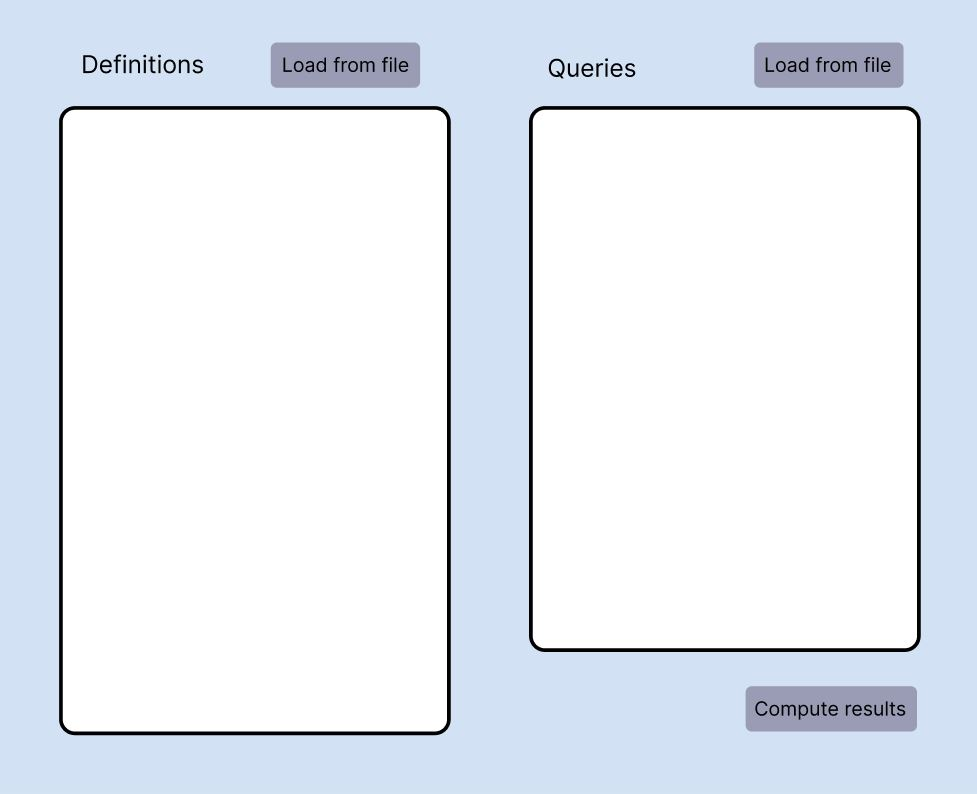
\includegraphics[width=\textwidth]{images/main_view.JPG}
    \caption{ Główny widok aplikacji }
    \label{fig:main_view}
\end{figure}

\begin{figure}[H]
    \centering
    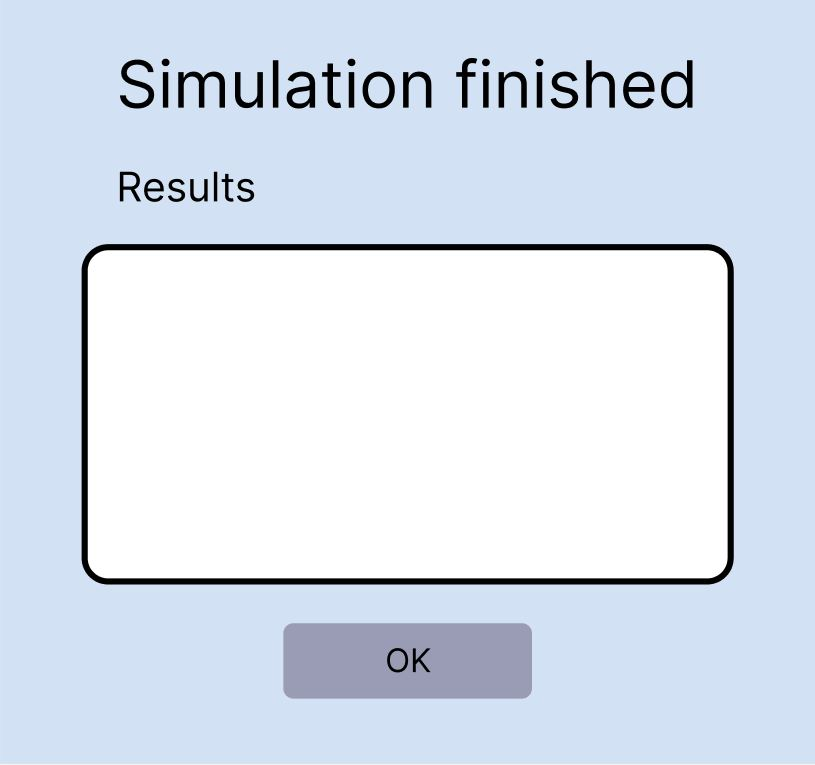
\includegraphics[width=0.6\textwidth]{images/success.JPG}
    \caption{ Dialog wynikowy }
    \label{fig:success}
\end{figure}

\begin{figure}[H]
    \centering
    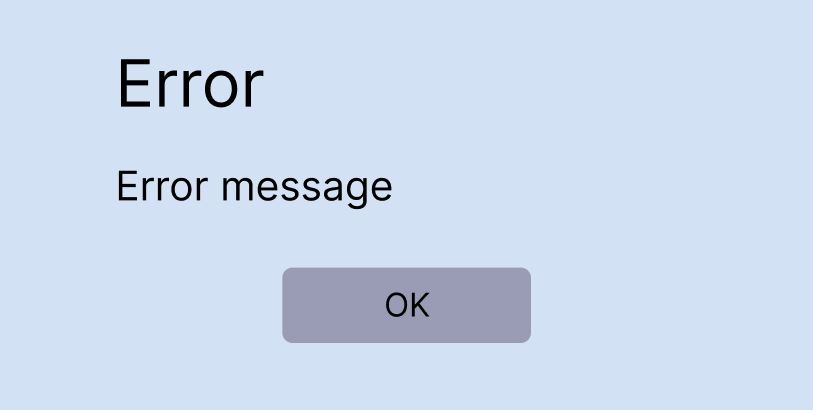
\includegraphics[width=0.6\textwidth]{images/error.JPG}
    \caption{ Dialog przedstawiający błąd }
    \label{fig:error}
\end{figure}


\section{Bibliografia}

\end{document}